\documentclass[12pt]{article}

\usepackage[margin = .8in]{geometry}
\usepackage{amsmath}
\usepackage{graphicx}
\usepackage{multicol, enumerate, tabularx}

\usepackage{adjustbox, soul, setspace}

\usepackage{fancyhdr}
\pagestyle{fancy}

\lhead{Math F113X: Numbers and Society}
\rhead{Lecture Notes}

\usepackage{tikz}
\usetikzlibrary{calc,trees,positioning,arrows,fit,shapes,through, backgrounds}
\usetikzlibrary{patterns}

\usetikzlibrary{decorations.markings}
\usetikzlibrary{arrows}

\usepackage{pgfplots}

\usepackage{longtable}
\usepackage{tabularx}

\newcommand{\ds}{\displaystyle}
\newcommand{\ans}[1][1in]{\rule{#1}{.5pt}}

\newcommand{\points}[1]{(#1 points.)}		% Trying to be lazy.

\usepackage{array}
\newcolumntype{L}[1]{>{\raggedright\let\newline\\\arraybackslash\hspace{0pt}}m{#1}}
\newcolumntype{C}[1]{>{\centering\let\newline\\\arraybackslash\hspace{0pt}}m{#1}}
\newcolumntype{R}[1]{>{\raggedleft\let\newline\\\arraybackslash\hspace{0pt}}m{#1}}
\newcommand{\red}[1]{\textcolor{red}{#1}}

\newcommand{\be}{\begin{enumerate}}
\newcommand{\ee}{\end{enumerate}}

\begin{document}
\begin{center}
{\large  Intro Sheet: Pivot Tables}
\end{center}
{\bf Goal:} Learn how to use a pivot table to summarize data

\subsection*{Instructions for setting up a pivot table}
\be
\item Get your data set into a spreadsheet. In this class, we will use the data set that is posted in Canvas. Your data needs to have headers at the top of each column, and there need to be no missing entries in the column.
\item Select your entire data set, by cells, including the column headers.
\item Select ``Summarize with Pivot Table'' or something similar. In Google Sheets, this is located in {\tt Insert > Pivot Table}. In Excel for Mac, {\tt Data Menu > Summarize With Pivot Table}. In Excel for Windows, using the toolbars at the top, maybe the {\tt Insert} tab on the toolbar, and then PivotTable is to the left?
\item Put your pivot table in a new worksheet. 
\item Use the headers to decide what to put in the rows and columns of your table, and what values you want to count up. In our example, we will have the Value be course enrollment, and we will put various things in the rows and columns.
\ee

\subsection*{Getting some data}
\be
\item Download the .csv file {\tt PivotTableDataSets - 2024-5-math-stat.csv} from Canvas, in the Activity 24 page. Click on the little icon next to it to download.

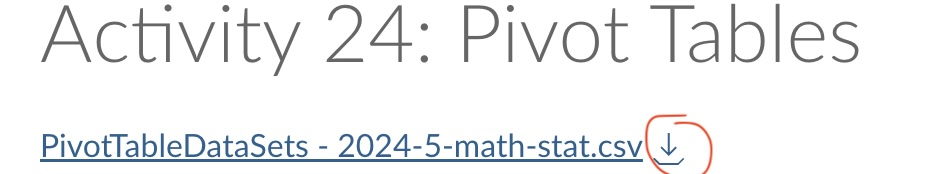
\includegraphics[width=3in]{Download.jpg}

Figure out how to open it in Google Sheets (or your spreadsheet of choice). One possibility is the following: 

Go to Google Drive, click the {\tt + New} button, click File Upload, navigate to where you saved the .csv you just downloaded, and after it uploads, click on the file you just uploaded to Drive. It should open in a Google Sheets page.

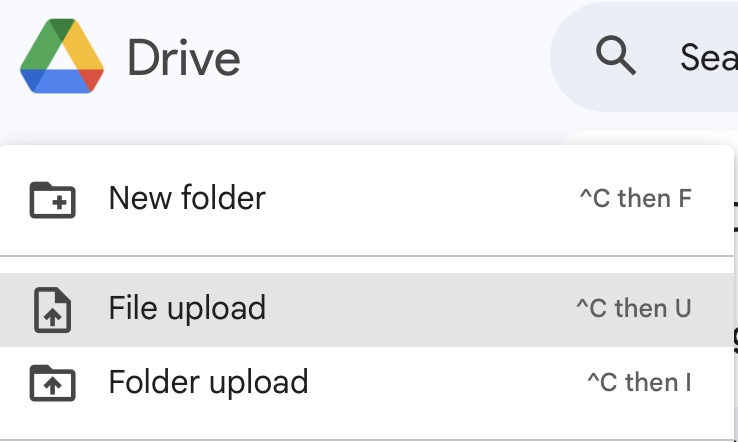
\includegraphics[width=2in]{upload.jpg} \hspace{1cm} 
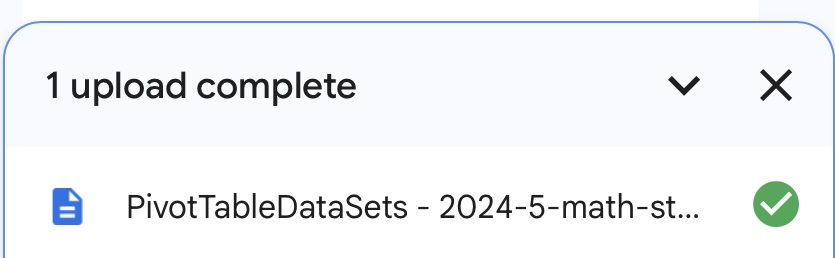
\includegraphics[width = 2in]{OpenInSheets.jpg}

\subsection*{Analyzing the data}

\be
\item Select the data cells in your spreadsheet and go to {\tt Insert > Pivot Table}. When it asks, create it in a New Sheet.

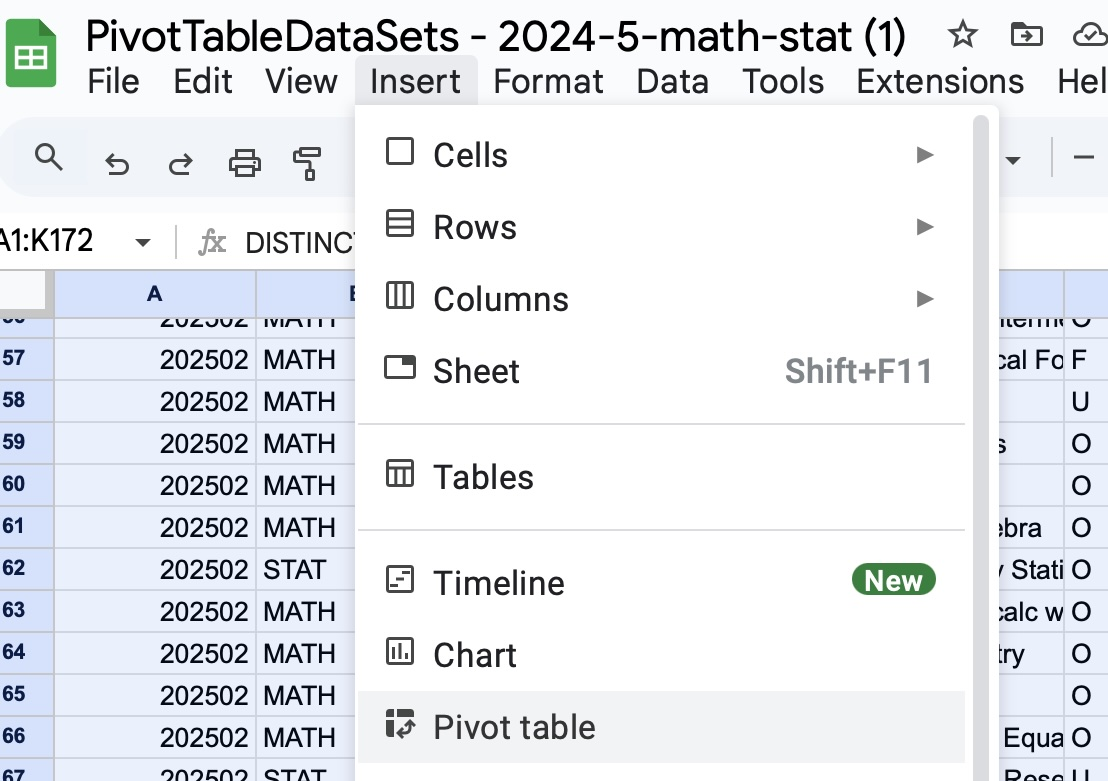
\includegraphics[width = 3in]{InsertPivotTable.jpg}

\item 
\be
\item Under {\tt Rows}, click {\tt Add} and then {\tt COURSE\_TITLE}. 
\item Under Columns, {\tt Add} and then {\tt DISTINCT COURSE\_TERM\_CODE}.
\item Under {\tt Values}, add {\tt COURSE\_ENROLLMENT}.
\ee

\item What does this Pivot Table tell us? The semester code 202403 means Fall 2024, 202501 means Spring 2025, and 202502 means Summer 2025.

\vfill

How many students took Numbers and Society in Spring 2025? \ans How many students took Numbers and Society in total? \ans

\item Under Rows, Add {\tt COURSE\_INSTRUCTOR}. How does the pivot table change? What does it tell us?

\vfill

How many instructors taught Numbers and Society in Spring 2025? \ans

\item Go to Rows, and click and drag to change the order of the items so that {\tt COURSE\_INSTRUCTOR} is above {\tt COURSE\_TITLE}. Now what does the pivot table tell you?

\ans

\item Add another Column, {\tt CourseAbbrv}. What happens? Change the order of {\tt CourseAbbrv} and {\tt DISTINCT COURSE\_TERM\_CODE}. Now what does the pivot table tell us?

\vfill

\item Click the X to delete {\tt COURSE\_INSTRUCTOR} from Rows and instead put in {\tt COURSE\_SUBJ\_CODE}. Now what is this pivot table counting?
\vspace{1in}


\item What happens if you delete {\tt COURSE\_TITLE} from Rows as well?

\vfill



\ee

\end{enumerate}
\end{document}
